\documentclass[twoside, 11pt]{article}
\usepackage[paperwidth=170mm, paperheight=240mm, left=20mm, right=18mm, top=18mm, bottom=18mm]{geometry}
\usepackage{ktu_dissertation_style}
\usepackage[
  backend=biber,
  bibstyle=iso-numeric,
  citestyle=numeric-comp,
  sorting=none,
  giveninits=true,
  doi=true,
  url=true,
  isbn=true
]{biblatex}
\renewcommand*{\multinamedelim}{\addcomma\space}
\renewcommand*{\finalnamedelim}{\addcomma\addspace and\space}
\addbibresource{references.bib}
\AtBeginBibliography{\fontsize{10pt}{12pt}\selectfont}

\usepackage[acronym,nonumberlist]{glossaries}
\newglossary[slg]{symbolslist}{syi}{syg}{List of Symbols}

\setglossarystyle{list}
\renewcommand{\glsgroupskip}{}

\renewcommand*{\glossentry}[2]{%
  \item[\glsentryitem{#1}\glstarget{#1}{\glossentryname{#1}}] -- \glossentrydesc{#1}.%
}
\makeglossaries
\begin{document}
\selectlanguage{english}
% =========================
% Acronyms
% =========================

\newacronym{aad}{AAD}{acoustic anomaly detection}
\newacronym{ai}{AI}{artificial intelligence}
\newacronym{cnn}{CNN}{convolutional neural network}
\newacronym{dl}{DL}{deep learning}
\newacronym{dnn}{DNN}{deep neural network}
\newacronym{dtl}{DTL}{deep transfer learning}
\newacronym{eg}{e.g.}{\textit{exempli gratia}}
\newacronym{emd}{EMD}{empirical mode decomposition}
\newacronym{esc}{ESC}{environmental sound classification}
\newacronym{etal}{et al.}{\textit{et alia}}
\newacronym{etc}{etc.}{\textit{et cetera}}
\newacronym{fft}{FFT}{fast Fourier transform}
\newacronym{ie}{i.e.}{\textit{id est}}
\newacronym{mlr}{MLR}{methodological literature review}
\newacronym{nlr}{NLR}{narrative literature review}
\newacronym{rnd}{R\&D}{research and development}
\newacronym{slr}{SLR}{systematic literature review}
\newacronym{snr}{SNR}{signal-to-noise ratio}
\newacronym{sota}{SOTA}{state of the art}
\newacronym{tlr}{TLR}{traditional literature review}

% =========================
% Terms / concepts / datasets / models
% =========================

\newglossaryentry{chromastft}{name={chroma-STFT}, description={a common lossy audio feature that compresses the full frequency spectrum of a signal into 12 bins, each corresponding to one of the twelve pitch classes of the Western scale. The acronym stands for "chroma short term Fourier transform"}}
\newglossaryentry{esc50}{name={ESC-50}, description={a dataset of 2,000 environmental audio clips across 50 categories, created as a standard benchmark for environmental sound classification methods}}
\newglossaryentry{fsc22}{name={FSC22}, description={a public benchmark dataset for detecting and classifying forest audio, particularly sounds linked to illegal activities like poaching and logging. "FSC" stands for "Forest Sound Classification," and "22" indicates the year of creation}}
\newglossaryentry{melspectrogram}{name={mel-spectrogram}, description={a time–frequency representation of audio that replaces the linear Hertz scale with the non-linear mel scale, reflecting human pitch perception}}
\newglossaryentry{mfcc}{name={MFCC}, description={a set of characteristics that represent the short-term power spectrum of a sound, based on the ear’s non-linear, logarithmic way of perceiving frequency. MFCC stands for "Mel-Frequency Cepstral Coefficients"}}
\newglossaryentry{mimii}{name={MIMII}, description={a publicly available collection of industrial machine audio created for unsupervised detection of abnormal sounds. its name is an acronym for "Malfunctioning Industrial Machine Investigation and Inspection"}}
\newglossaryentry{stft}{name={STFT}, description={an abbreviation of "Short-Time Fourier Transform," a mathematical method for analyzing how the frequency and phase content of short segments of a signal vary over time}}

% =========================
% Symbols
% =========================

\newglossaryentry{disctime}{name={$n$}, description={discrete-time frame index}, type=symbolslist, sort=n, first={discrete-time frame index ($n$)}}%
\newglossaryentry{fftsize}{name={$N$}, description={fast Fourier transform size}, type=symbolslist, sort=nfftsize, first={\gls{fft} size ($N$)}}%
\newglossaryentry{frequency}{name={$f$}, description={frequency bin}, type=symbolslist, sort=f, first={frequency bin ($f$)}}%
\newglossaryentry{hoplen}{name={$H$}, description={hop length}, type=symbolslist, sort=hoplen, first={hop length ($H$)}}%
\newglossaryentry{inputsignal}{name={$x[n]$}, description={discrete-time input signal}, type=symbolslist, sort=xn, first={discrete-time input signal ($x[n]$)}}%
\newglossaryentry{slidwinfunc}{name={$\omega[n - tH]$}, description={sliding-window function}, type=symbolslist, sort=omegah, first=sliding-window function ($\omega[n - tH]$)}%
\newglossaryentry{spectrogram}{name={$X[t, f]$}, description={spectrogram}, type=symbolslist, sort=xtf, first={spectrogram ($X[t, f]$)}}%
\newglossaryentry{time}{name={$t$}, description={time}, type=symbolslist, sort=time}%

\clearpage
% \input{TitlePageRev}
\definecolor{lines_name}{RGB}{212,175,54}

\begin{titlepage}
   \begin{center}
   	 

   	%\includegraphics[width=2.46cm\textwidth]{university}
        % \vspace*{0.3cm}
        % \includegraphics[width=2.46cm]{images/ktu-ikona.pdf}
        % \vspace{0.3cm}

       \MakeUppercase{\Large {Kaunas University of Technology}}\\
       \vspace{5cm}
       \MakeUppercase{\Large Name Surname}\\
       \vspace{2cm}
       \huge
        \expandafter\expandafter\MakeUppercase{Your Title In English}\\
        \large
        \vspace{3cm}
        	{\large Doctoral Dissertation} \\
            {\large {Study Field, Study Area (CODE)}}
            %{\projectFaculty, \projectStudies}

       \vfill
       
       
      \large{{\the\year, Kaunas}}
   \end{center}
   \pagebreak
   \thispagestyle{empty}
\noindent The dissertation has been prepared at the Department of Software Engineering of the Faculty of Informatics of Kaunas University of Technology in 2021–2025.\\

\noindent The doctoral right has been granted to Kaunas University of Technology together with Vilnius Gediminas Technical University.\\

\noindent \textbf{Research supervisor:}\\
Prof. Dr. Name SURNAME (Kaunas University of Technology, Technological Sciences, Informatics Engineering, T 007).\\

\noindent \textbf{Edited by:} English language editor Name SURNAME (Publishing House Technologija), Lithuanian language editor Name SURNAME (Publishing House Technologija).\\

\noindent \textbf{Dissertation Defence Board of Informatics Engineering Science Field:}\\
Prof. Dr. Name SURNAME (Kaunas University of Technology, Technological Sciences, Informatics Engineering, T 007) – \textbf{chairperson};\\
Prof. Dr. Name SURNAME (Vilnius Gediminas Technical University, Technological Sciences, Informatics Engineering, T 007);\\
Assoc. Prof. Dr. Name SURNAME (Linnaeus University, Sweden, Technological Sciences, Informatics Engineering, T 007);\\
Prof. Dr. Name SURNAME (Kaunas University of Technology, Technological Sciences, Measurement Engineering, T 010);\\
Prof. Dr. Name SURNAME (Vilnius Gediminas Technical University, Technological Sciences, Informatics Engineering, T 007).\\

\noindent The dissertation defence will be held on 28 April 2026, at 10:30 a.m. at the Rectorate Hall of Kaunas University of Technology in the meeting of the Dissertation Defence Board of the Informatics Engineering Science Field.\\

\noindent Address: K. Donelaičio 73-402, LT-44249 Kaunas, Lithuania.\\ 
Phone: +370 608 28 527; e-mail doktorantura@ktu.lt\\

\noindent The dissertation was sent out on 27 March 2026.\\
The dissertation is available on the website http://ktu.edu, at the library of Kaunas University of Technology (Gedimino 50, Kaunas) and Vilnius Gediminas Technical University (Saulėtekio 14, Vilnius).

   \vfill

   \noindent \textcopyright\ N. Surname, \the\year


\end{titlepage}

\clearpage
\definecolor{lines_name}{RGB}{212,175,54}
\begin{titlepage}
   \begin{center}
   	 

   	%\includegraphics[width=2.46cm\textwidth]{university}
        % \vspace*{0.3cm}
        % \includegraphics[width=2.46cm]{images/ktu-ikona.pdf}
        % \vspace{0.3cm}

       \MakeUppercase{\Large {Kauno Technologijos Universitetas}}\\
       \vspace{5cm}
       \MakeUppercase{\Large Vardas Pavardė}\\
       \vspace{2cm}
       \huge
        \expandafter\expandafter\MakeUppercase{Jūsų pavadinimas lietuvių kalba} \\
        \large
        \vspace{3cm}
        	{\large Daktaro disertacija} \\
            {\large Jūsų studijų sritis, Jūsų studijų area (kodas)}

       \vfill
       
       
      \large{{\the\year, Kaunas}}
   \end{center}
   \pagebreak
   \thispagestyle{empty}
   \noindent Disertacija rengta 2021–2025 metais Kauno technologijos universiteto Informatikos fakultete, Programų inžinerijos katedroje.\\
   
   \noindent Doktorantūros teisė Kauno technologijos universitetui suteikta kartu su Vilniaus Gedimino technikos universitetu.\\
   
   \noindent \textbf{Mokslinis vadovas:}\\
   prof. dr. Vardas PAVARDĖ (Kauno technologijos universitetas, technologijos mokslai, informatikos inžinerija, T 007).\\
   
   \noindent \textbf{Redagavo:} anglu˛ kalbos redaktorius Vardas PAVARDĖ (leidykla „Technologija“), lietuviu˛ kalbos redaktorė Vardas PAVARDĖ (leidykla „Technologija“).\\
   
   \noindent \textbf{Informatikos inžinerijos mokslo krypties disertacijos gynimo taryba:}\\
   prof. dr. Vardas PAVARDĖ (Kauno technologijos universitetas, technologijos mokslai, informatikos inžinerija, T 007) – \textbf{pirmininkas};\\
   prof. dr. Vardas PAVARDĖ (Vilniaus Gedimino technikos universitetas, technologijos mokslai, informatikos inžinerija, T 007);\\
   doc. dr. Vardas PAVARDĖ (Linėjaus universitetas, Švedija, technologijos mokslai, informatikos inžinerija, T 007);\\
   prof. dr. Vardas PAVARDĖ (Kauno technologijos universitetas, technologijos mokslai, matavimų inžinerija, T 010);\\
   prof. dr. Vardas PAVARDĖ (Vilniaus Gedimino technikos universitetas, technologijos mokslai, informatikos inžinerija, T 007).\\
   
   \noindent Disertacija bus ginama viešame Informatikos inžinerijos mokslo krypties disertacijos gynimo tarybos posėdyje 2026 m. balandžio 28 d. 10:30 val. Kauno technologijos universiteto Rektorato salėje.\\
   
   \noindent Adresas: K. Donelaičio g. 73-402, LT-44249 Kaunas, Lietuva.\\
   Tel: +370 608 28 527; el. paštas doktorantura@ktu.lt\\
   
   \noindent Disertacija išsiųsta 2026 m. kovo 27 d.\\
   Su disertacija galima susipažinti interneto svetainėje http://ktu.edu, Kauno technologijos universiteto bibliotekoje (Gedimino g. 50, Kaunas) ir Vilniaus Gedimino technikos universiteto bibliotekoje (Saulėtekio al. 14, Vilnius).

   \vfill

   \noindent \textcopyright\ V. Pavardė, \the\year


\end{titlepage}

\clearpage
 %to include title page in page numbering counter
\setcounter{page}{5}
\renewcommand{\contentsname}{\textbf{\MakeUppercase{Table of Contents}}}
\tableofcontents
\clearpage
\addcontentsline{toc}{section}{\listtablename}
\listoftablesnospace
\clearpage
\clearpage
\addcontentsline{toc}{section}{\listfigurename}
\listoffiguresnospace
\section*{\textbf{\MakeUppercase{List of Abbreviations and Terms}}}
\addcontentsline{toc}{section}{\MakeUppercase{List of Abbreviations and Terms}}

\vspace{1em}
\noindent\textbf{Abbreviations:}\vspace{-1.5em}

\begingroup
\GlossSemicolon
\let\clearpage\relax
\let\cleardoublepage\relax
\printglossary[type=\acronymtype, title={}]
\endgroup

\vspace{1.5em}
\noindent\textbf{Terms:}\vspace{-1.5em}

\begingroup
\GlossPeriod
\let\clearpage\relax
\let\cleardoublepage\relax
\printglossary[type=main, title={}]
\endgroup

%% Uncomment this section to print the list of symbols, and remember to update the heading. 
% \vspace{2em}
% \noindent\textbf{Symbols:}\vspace{-2em}

% \begingroup
% \GlossSemicolon
% \let\clearpage\relax
% \let\cleardoublepage\relax
% \printglossary[type=symbolslist, title={}]
% \endgroup
\clearpage
\addcontentsline{toc}{section}{\MakeUppercase{Introduction and Research Motivation}}
\section*{\MakeUppercase{Introduction and Research Motivation}}\label{chap:intro}
\glsresetall
\glsunset{etal}
\glsunset{eg}
\glsunset{etc}
\glsunset{ie}
\subsection*{Relevance of the Work}\label{subsec:relevance}
Audio classification plays a crucial role in contemporary \gls{aad} systems by providing {essential insights}\label{rev:ru_min_1a} suitable for various applications~\cite{Kilickaya2025, LoScudo2023, Barusco2025}. These fields are valid not only for industrial environments~\cite{Purohit2019} but also for dynamic urban areas~\cite{Piczak2015, Salamon2014} and even complex natural ecosystems, such as forests~\cite{Bandara2023}. \dots

\dots

\subsection*{Formulation of Problems}\label{sec:form_prob}
Audio-based classification has strong potential in many domains, but recurring issues still obstruct its effective use in real-world data collection and processing. These issues are particularly critical when \dots

\begin{enumerate}[leftmargin=*]
	\item Although handcrafted audio features like \gls{mfcc} and chroma-based representations are widely used, there is still no systematic understanding of \dots
	\item \dots
\end{enumerate}

\subsection*{Aim of the Research}\label{sec:aim}
{This research aims to improve the accuracy, robustness, and reliability of \gls{aad} in noisy environments. It focuses on better \dots}

\subsection*{Research Objectives}\label{sec:r_o}
The overarching goal of this study is to enhance the accuracy, robustness, and dependability of \dots

\begin{enumerate}[leftmargin=*]
    \item To review and integrate prior work on \gls{aad} and \gls{esc}, focusing on feature representations, \gls{dnn} models, and evaluation methods in noisy environments.
    
    \item \dots
\end{enumerate}

\subsection*{Scientific Novelty}\label{subsec:sci_nov}
This research introduces several significant scientific contributions that \dots

\begin{enumerate}[leftmargin=*]
	\item {A key advancement is the full use of the \gls{mimii} dataset across all devices and \gls{snr} levels, unlike prior work restricted to specific devices or \dots}
	\item \dots
\end{enumerate}


\subsection*{Practical Significance}\label{subsec:1_7}
\begin{enumerate}[leftmargin=*]
	\item Applying \gls{dl} to acoustic-based anomaly detection is a promising approach for \dots
	\item \dots
\end{enumerate}

\subsection*{Dissertation Statements} \label{subsec:des_state}
\begin{enumerate}[leftmargin=*]
	\item {The major class imbalance in the \gls{mimii} dataset was addressed using \dots}
	
	\item \dots
\end{enumerate}

\subsection*{Scientific Approvals} \label{sec:scie_app}
{To validate and support the methodology developed in this doctoral research, five scientific contributions have been produced over the past four years. These consist of \dots}

\subsubsection*{Articles indexed in Web of Science and Scopus}
\begin{enumerate}[leftmargin=*]
	\item Ahmad Qurthobi, Rytis Maskeli\={u}nas, and Robertas Dama\v{s}evi\v{c}ius. Detection of mechanical failures in \dots
	\item \dots
\end{enumerate}
\subsubsection*{International conference proceedings}
\begin{enumerate}[leftmargin=*]
	\item Ahmad Qurthobi and Rytis Maskeli\={u}nas. The effect of augmentation and filtration on noisy environment’s acoustic signals to detect abnormalities in \dots
	\item \dots
\end{enumerate}

\subsection*{Dissertation Structure}\label{sec:dis_struc}
This dissertation is structured into five chapters. Chapter~\hyperref[chap:intro]{\MakeUppercase{Introduction and Research Motivation}} presents \dots

\clearpage
\section{\MakeUppercase{Literature Reviews}} \label{chap:one}
This chapter presents the evolution of research on \gls{dnn} in acoustics and its application to event detection, environmental monitoring, etc. Section \ref{sec:fe_and_dnn} examines the progression of audio usage in \gls{ai}, focusing on time-frequency feature extraction methods and \gls{dnn} learning models based on \gls{cnn} and attention mechanisms. Section \ref{sec:acc_mon} outlines \dots

\subsection{Audio Feature Extraction and Deep Neural Networks for Acoustic Classification}\label{sec:fe_and_dnn}
\begin{figure}[!ht]
    \centering
    \begin{subfigure}[b]{0.45\textwidth}
	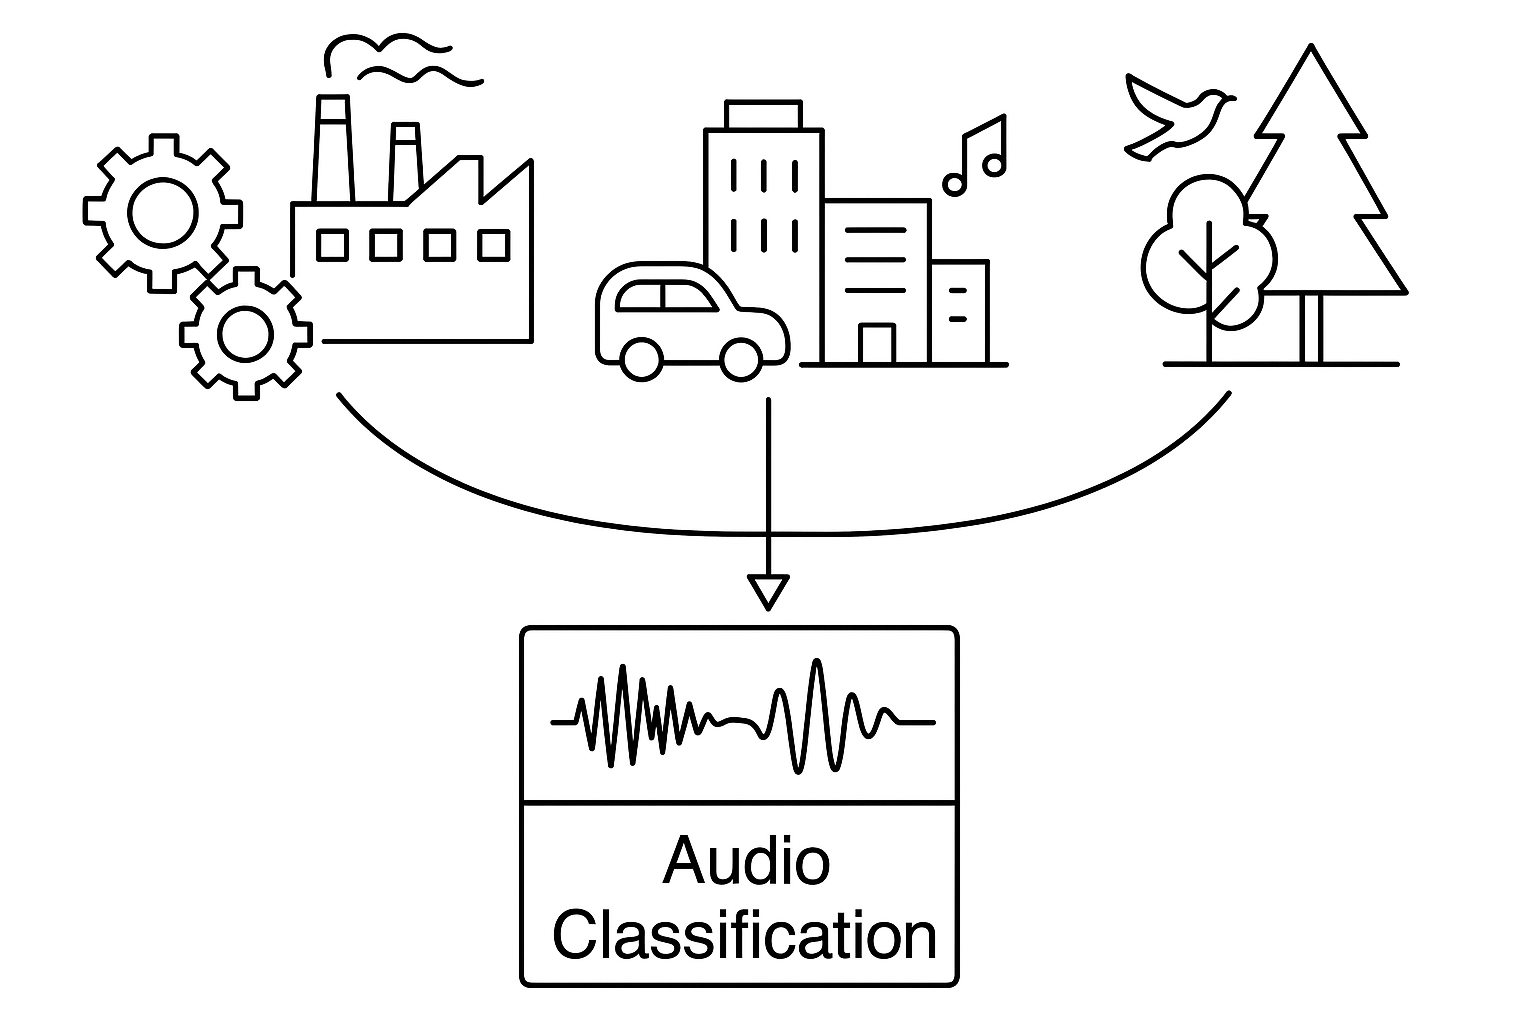
\includegraphics[width=\textwidth]{images/sketch/audioclassification.png}
	\caption{sketch}
	\label{fig:audio-based}
\end{subfigure}
\hfill
\begin{subfigure}[b]{0.45\textwidth}
	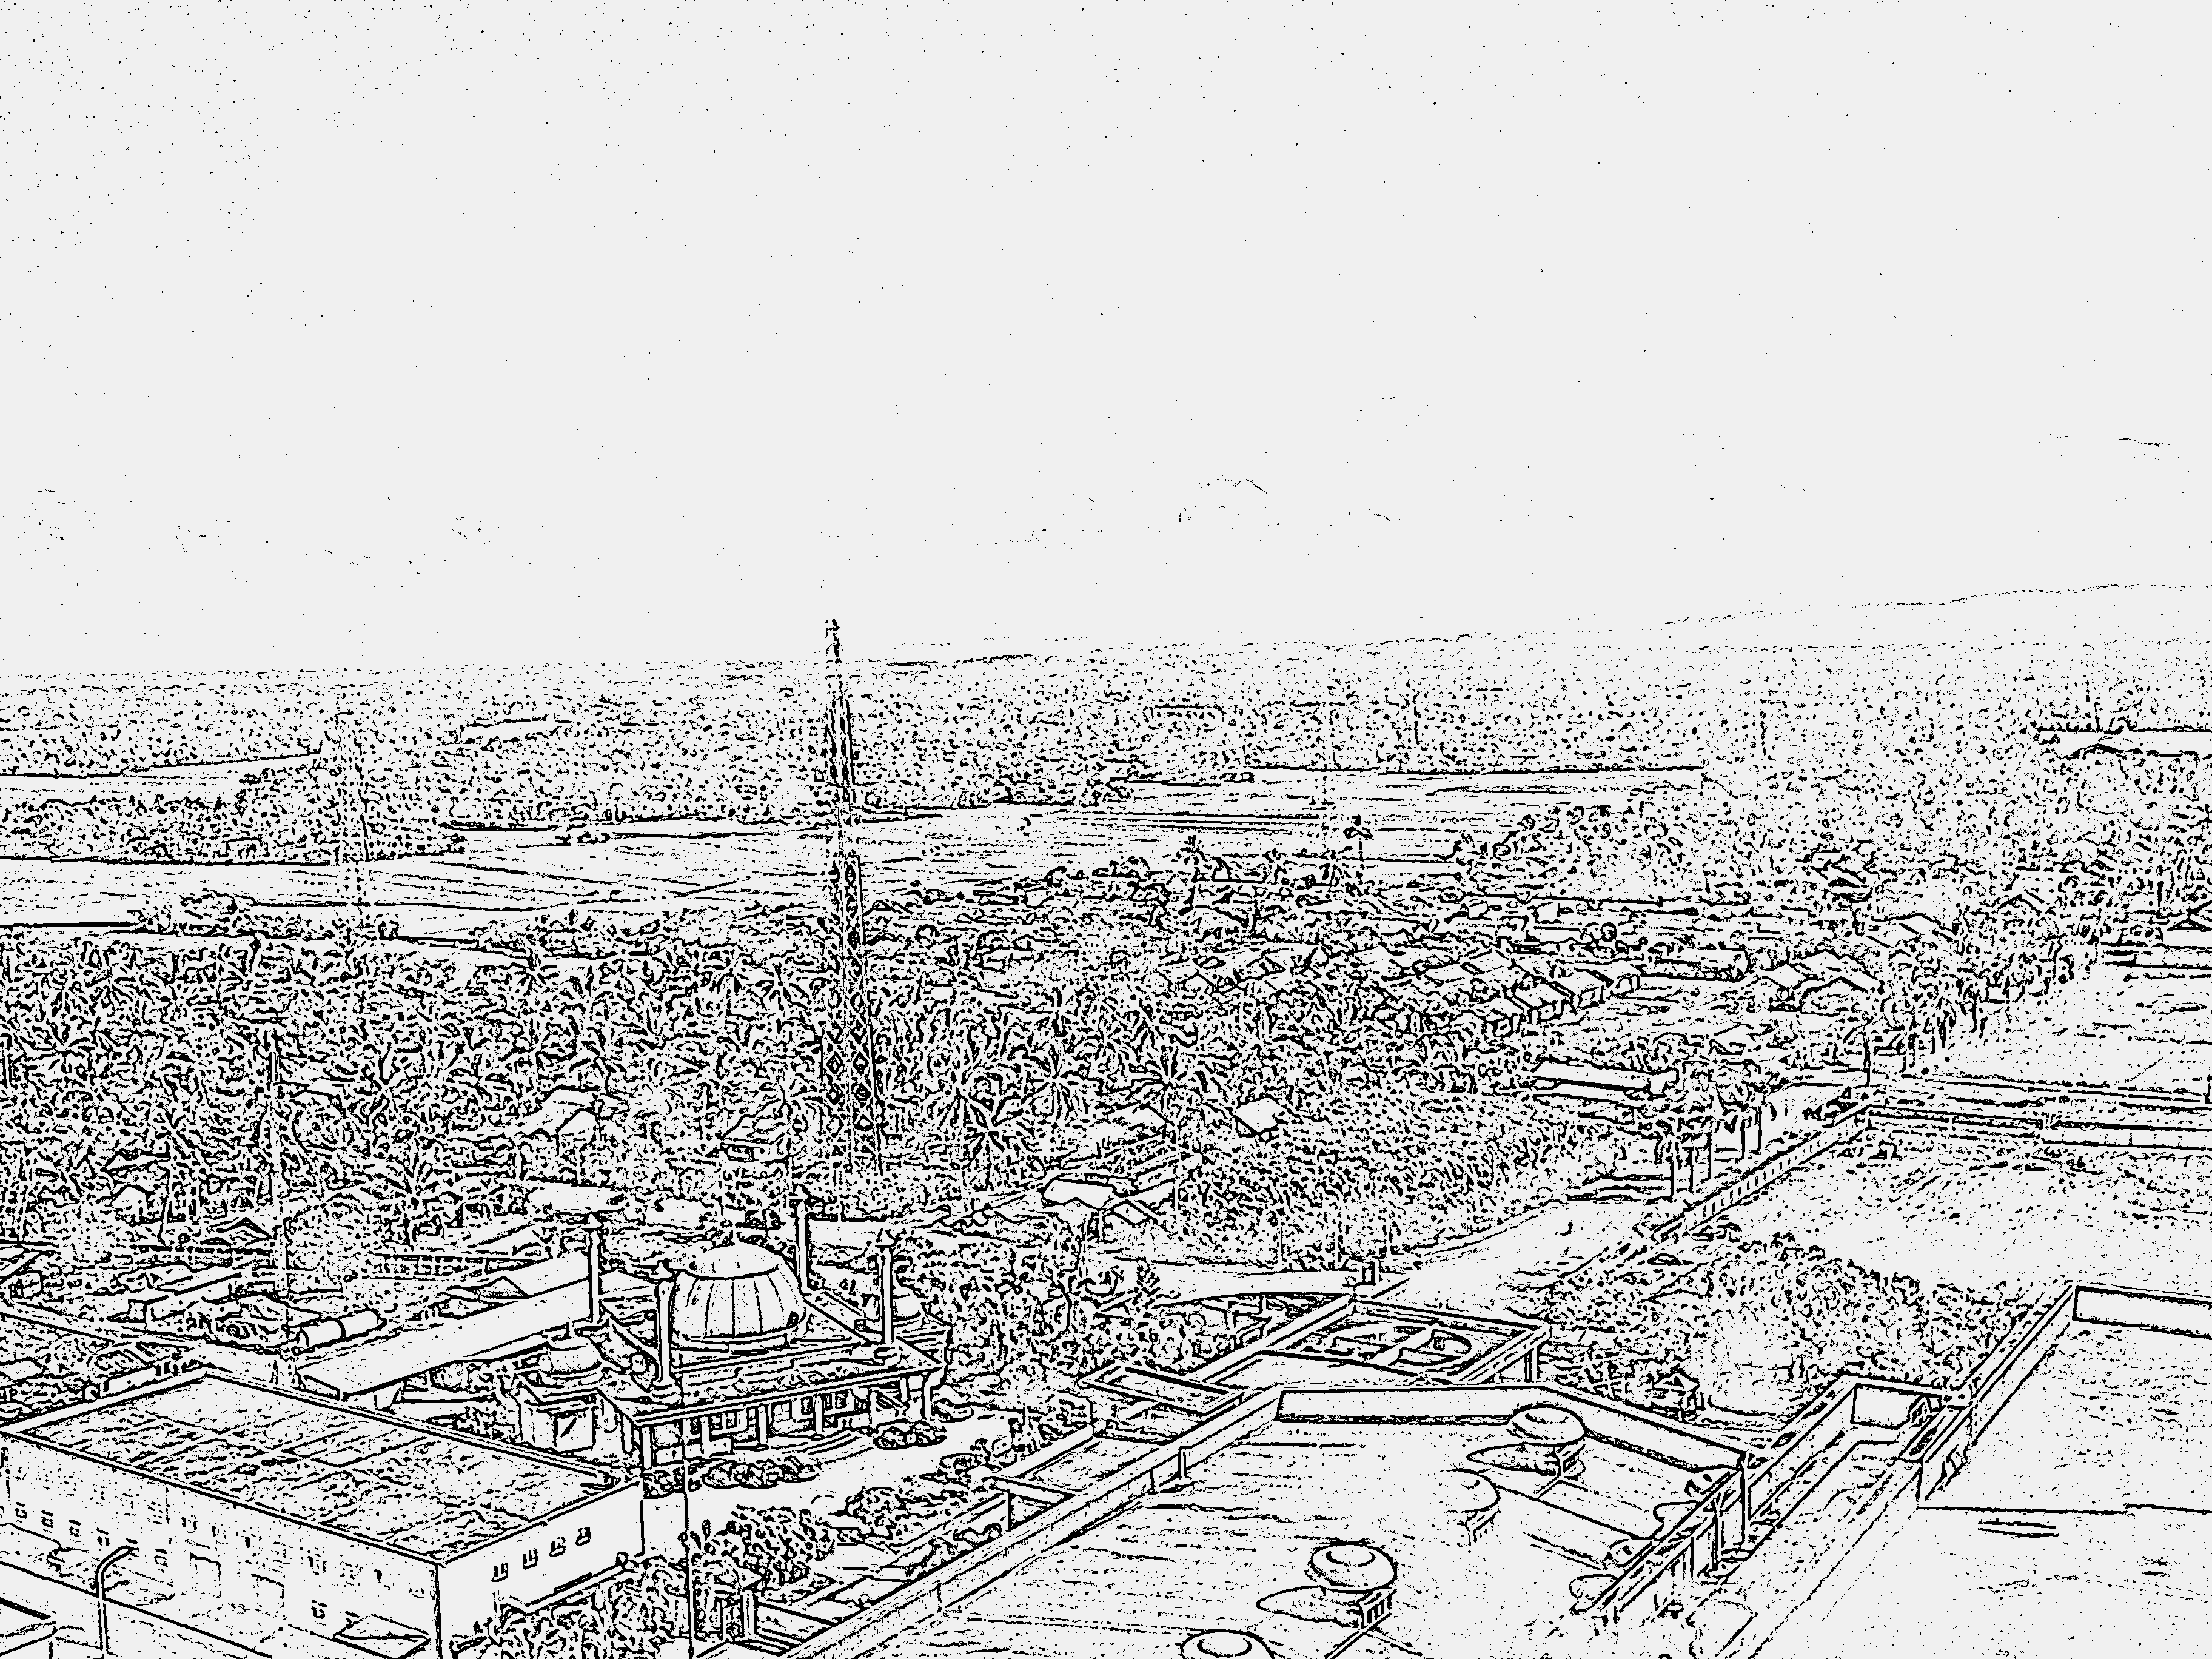
\includegraphics[width=\linewidth]{images/sketch/all_environment_sketch.png}
	\caption{real environment}
	\label{fig:audio_based}
\end{subfigure}
    \caption{Illustration of the implementation of audio-driven classification}
    \label{fig:illustration}
\end{figure}

A combined analysis of advances in \gls{ai} methods and new datasets is essential for \dots

\dots

These developments unlock the potential to broaden the scope of audio classification, enabling both the detection of specific anomalies in varied applications and the identification of unexpected events in real environments. Figure~\ref{fig:illustration} provides \dots


\subsection{Acoustic Monitoring in Noise: Application Areas, Noise Profiles, and Anomaly Definition} \label{sec:acc_mon}
The utilization of acoustic methods in the context of environmental surveillance or the identification of irregularities, as illustrated in Figure~\ref{fig:audio_based}, boasts a substantial historical precedent~\cite{Simonovic2021, Vicuna2017}. In general, abnormal conditions that occur at the measuring device or location can be detected by \dots

\dots

\subsection{Evolution of Acoustic Anomaly Detection Research: A Review Perspective} \label{sec:evo_and}
The merging of acoustic methods with the progress in \gls{ai} has garnered growing attention from researchers, particularly in their use for anomaly detection. The timeline of progress in this interdisciplinary area is detailed through multiple reviews (\gls{tlr}, \gls{slr}, \gls{mlr}, \gls{nlr}, \gls{etc}) that together explain the development, usage, and effectiveness of these techniques in different fields. Table~\ref{tab:recent_literature_reviews} offers a compiled overview of these important reviews.

\glsunset{dtl}
\begin{table}[!ht]
	\centering
	\caption{Recent literature reviews in acoustic-based detections}
	\label{tab:recent_literature_reviews}
    \small
	\begin{tabular}{p{0.3\linewidth}ccp{0.4\linewidth}}
		\toprule
		\multicolumn{1}{c}{Author(s)}&\multicolumn{1}{c}{Method}&Citations&\multicolumn{1}{c}{Focus of study}\\
		\midrule
		Shaikh \gls{etal} (2021)~\cite{Shaikh2021} & \gls{tlr} & 44 & Exploring the potential of acoustic signal analysis in facilitating machine fault diagnosis.\\
		\hline
		Qurthobi \gls{etal} (2022)~\cite{Qurthobi2022}& \gls{slr} & 52 & \Gls{sota} mechanical failure detection using acoustic methods.\\
		\hline
		\dots& \dots & \dots & \dots\\
		\bottomrule
	\end{tabular}
\end{table}
\glsreset{dtl}
\dots

\clearpage
\section{\MakeUppercase{Datasets and Methodologies}} \label{chap:two}
This chapter presents the materials and methods used to develop and evaluate the proposed framework for audio classification and anomaly detection. Section~\ref{sec:datasets} describes the datasets used in this study, emphasizing their acoustic characteristics and relevance to industrial, urban, and natural environments. Section~\ref{sec:feature_extractors} introduces \dots
\subsection{Datasets}\label{sec:datasets}
To thoroughly evaluate audio classification systems, it is essential to test them across various acoustic environments. Thus, three well-known and publicly accessible datasets (\gls{ie}, \gls{esc50}, \gls{mimii}, and \gls{fsc22}) were chosen, each representing \dots
\glsreset{mimii}

\subsection{Feature Extractors}\label{sec:feature_extractors}
To ensure strong and precise audio classification, a collection of commonly used and perceptually inspired feature extraction techniques was employed. In particular, \gls{melspectrogram}, \gls{mfcc}, and \gls{chromastft} representations were calculated for \dots

\dots
\glsreset{melspectrogram}
\subsubsection{Melspectrogram}
\dots

\begin{equation}
	X[t, f] = \sum_{n=0}^{N-1} x[n] \, \omega[n - tH] \, \exp\left(-j 2\pi \frac{f n}{N}\right) \label{eq:stftmel}
\end{equation}

Equation~(\ref{eq:stftmel}) computes the \gls{stft} of the \gls{inputsignal} by applying a \gls{slidwinfunc} to successive, overlapping frames of the signal. This segmentation is determined by parameters such as \gls{time}, \gls{frequency}, \gls{disctime}, \gls{fftsize}, and \gls{hoplen}. Each windowed segment is subsequently transformed into the frequency domain via a complex exponential kernel, yielding a time–frequency representation in the form of a \gls{spectrogram}. Each element of this complex-valued matrix encodes the spectral content corresponding to a specific \gls{frequency} and \gls{time} frame, thereby capturing the localized frequency structure of the signal over time.

\begin{equation}
	S_{\mathrm{P}}[t, f] = \left| X[t, f] \right|^2
	\label{eq:powerspec}
\end{equation}

\dots

\clearpage
\section{\MakeUppercase{Performance Evaluation and Analysis}}\label{chap:three}
This chapter reports an experimental assessment of the proposed audio classification frameworks across varied acoustic settings, spanning industrial, urban, and natural soundscapes. Several public datasets are used to evaluate model robustness and generalization under heterogeneous, noisy conditions. Although anomaly event detection remains the core objective of this dissertation, benchmark datasets such as \gls{esc50} and \gls{fsc22}, which are typically framed as multi-class classification problems, are instead used as proxy testbeds to investigate anomaly-related characteristics, including resilience to background noise, detection of rare or short-duration events, and consistency across diverse sound classes.

\dots

% You need this part to separate between English and Lithuanian Part

\addtocontents{lof}{\protect\vspace*{2em}}
\addtocontents{lof}{\textbf{\MakeUppercase{Paveikslų sąrašas}}\par}
\addtocontents{lof}{\protect\vspace*{1em}}

\addtocontents{lot}{\protect\vspace*{2em}}
\addtocontents{lot}{\textbf{\MakeUppercase{Lentelių sąrašas}}\par}
\addtocontents{lot}{\protect\vspace*{1em}}

\clearpage
\addcontentsline{toc}{section}{\MakeUppercase{Conclusions and Future Works}}
\section*{\MakeUppercase{Conclusions and Future Works}}\label{chap:five}
% \glsresetall
\subsection*{Conclusions}\label{sec:conclusions}
\begin{enumerate}[leftmargin=*]
	\item \dots
    \item \dots
\end{enumerate}
\subsection*{Future Works}
\begin{enumerate}[leftmargin=*]
	\item \dots
	\item \dots
\end{enumerate}

\clearpage
\selectlanguage{lithuanian}
\addcontentsline{toc}{section}{\MakeUppercase{Santrauka}}
\noindent\begin{minipage}{\textwidth}
	\textbf{\MakeUppercase{Santrauka}}
    \setcounter{section}{0}
    % \addtocontents{toc}{\protect\setcounter{tocdepth}{0}}
	\subsection*{\k{I}vadas}\label{chap:introlt}
    % \addtocontents{toc}{\protect\setcounter{tocdepth}{2}}
\end{minipage}
\subsection*{Darbo aktualumas}
Garso klasifikavimas atlieka svarbų vaidmenį aptinkant anomalijas, nes suteikia vertingos informacijos įvairiais taikymo atvejais~\cite{Kilickaya2025, LoScudo2023, Barusco2025}. Šios sistemos yra naudingos pramoninėse ir miesto vietovėse~\cite{Purohit2019, Piczak2015, Salamon2014}, taip pat sudėtingose gamtinėse vietovėse, pvz., miškuose~\cite{Bandara2023}. Garso duomenys gali būti \dots

\dots
\subsection*{Problemų formulavimas}
\begin{enumerate}[leftmargin=*]
	\item \dots
	\item \dots
\end{enumerate}
\subsection*{Tyrimo tikslas}
Šio tyrimo tikslas – pagerinti garso pagrindu veikiančių anomalijų aptikimo sistemų tikslumą, patikimumą ir \dots

\subsection*{Tyrimo uždaviniai}
\begin{enumerate}[leftmargin=*]
	\item \dots
	\item \dots
\end{enumerate}

\subsection*{Mokslinės naujovės}
Šiame tyrime pristatomos šios mokslinės naujovės, kurios išplečia \dots

\begin{enumerate}[leftmargin=*]
	\item \dots
	
	\item \dots
\end{enumerate}

\subsection*{Praktinė reikšmė}
\begin{enumerate}[leftmargin=*]
	\item \dots
	\item \dots
\end{enumerate}

\subsection*{Disertacijos teiginiai}
\begin{enumerate}
	\item \dots
	\item \dots
\end{enumerate}

\subsection*{Moksliniai aprobavimai}
Šio disertacinio tyrimo metodologiją ir \dots

\subsection*{Disertacijos struktūra}

Disertaciją sudaro penki skyriai. \hyperref[chap:introlt]{„Įvadas“} skyriuje pristatoma tyrimo problema ir jos motyvacija, apibrėžiama šiame darbe vartojama akustinių anomalijų sąvoka ir pagrindžiamas pramoninių, urbanistinių bei miško garso aplinkų pasirinkimas kaip papildomų vertinimo sričių. \hyperref[chap:twolt]{„Literatūros apžvalgos apie giluminio neuroninio tinklo metodą akustinių anomalijų įvykiams aptikti“} skyriuje pateikiama \dots

\nopagebreak
\addtocontents{toc}{\protect\setcounter{tocdepth}{0}}
% \Needspace{4\baselineskip}
\subsection*{Literatūros apžvalgos apie giluminio neuroninio tinklo metodą akustinių anomalijų įvykiams aptikti}\label{chap:onelt}
% \addtocontents{toc}{\protect\setcounter{tocdepth}{2}}
Akustinių metodų naudojimas aplinkos stebėjimo ar pažeidimų nustatymo kontekste turi reikšmingą istorinį precedentą~\cite{Simonovic2021, Vicuna2017}. Paprastai neįprastos sąlygos stebimose įrangose gali būti nustatytos pagal pagamintų akustinių signalų savybių kitimą, pavyzdžiui, dažnio ir amplitudės pokyčius.~\cite{Holford2017, Cooper2020}. Akustinio metodo pranašumas, palyginti su kitais metodais, yra tai, kad \dots

\dots

\nopagebreak
\subsection*{Duomenų rinkiniai ir metodologija}\label{chap:twolt}
% \DeclareCaptionLabelFormat{rev}{#2~#1}
% \renewcommand{\figurename}{paveikslas}
% \renewcommand{\tablename}{lentelė}
% \renewcommand{\listfigurename}{Paveikslų sąrašas}
% \renewcommand{\listtablename}{Lentelių sąrašas}%
% \captionsetup[figure]{labelformat=ltrev}
% \captionsetup[table]{labelformat=ltrev}
\subsection*{Duomenų minkiniai}
% \glsreset{mimii}
\addtocontents{toc}{\protect\setcounter{tocdepth}{2}}
\subsubsection*{MIMII}
\addtocontents{toc}{\protect\setcounter{tocdepth}{4}}
% \glsreset{mimii}
\begin{table}[!ht]
	\centering
	% \footnotesize
	\caption[Garso failų pasiskirstymas MIMII duomenų rinkinyje]{Garso failų pasiskirstymas \gls{mimii} duomenų rinkinyje~\cite{Purohit2019}}
	% \captionsetup{labelformat=rev}
	\label{tab:mimii_datasetslt}
	\renewcommand{\arraystretch}{1.2}
	\small
	\begin{tabular}{|c|c|c|c|c|c|c|c|}
		\hline
		\multirow{2}{*}{\textbf{Įrenginys}} & \multirow{2}{*}{\textbf{ID}} & \multicolumn{2}{c|}{\textbf{Sąlyga}}&\multirow{2}{*}{\textbf{Įrenginys}} & \multirow{2}{*}{\textbf{ID}} & \multicolumn{2}{c|}{\textbf{Sąlyga}}\\
		\cline{3-4}
		\cline{7-8}
		&&\textbf{Normal} & \textbf{Abnormal}&&&\textbf{Normal} & \textbf{Abnormal}\\
		\hline
		\multirow{4}{*}{Fan} & id\_00 & 1011 & 407&\multirow{4}{*}{Slider} & id\_00 & 1068 & 356\\
		\cline{2-4}
		\cline{6-8}
		& id\_02 & 1016& 359&& id\_02 & 1068 & 267\\
		\cline{2-4}
		\cline{6-8}
		& id\_04 & 1033 & 348&& id\_04 & 534 & 178\\
		\cline{2-4}
		\cline{6-8}
		& id\_06 & 1015 &361&& id\_06 & 534 & 89\\
		\hline
		\multirow{4}{*}{Pump} & id\_00 & 1006 & 143&\multirow{4}{*}{Valve} & id\_00 & 991 & 119\\
		\cline{2-4}
		\cline{6-8}
		& id\_02 & 1005 & 111&& id\_02 & 708 & 120\\
		\cline{2-4}
		\cline{6-8}
		& id\_04 & 702 & 100&& id\_04 & 1000 & 120\\
		\cline{2-4}
		\cline{6-8}
		& id\_06 & 1036 & 102&& id\_06 & 992 & 120\\
		\hline
	\end{tabular}
\end{table}
\begin{table}[!ht]
	\centering
	\caption[Bendrosios MIMII duomenų rinkinio savybės]{Bendrosios \gls{mimii} duomenų rinkinio savybės~\cite{Purohit2019}}
	\label{tab:mimii_propertiesslt}
	\small
	\begin{tabular}{ll}
		\hline
		\multicolumn{1}{c}{\textbf{Nuosavybė}} & \multicolumn{1}{c}{\textbf{Value}} \\
		\hline
		Bendras failų skaičius & $\sim$55,000+ \\
		Failo trukmė & 10 sekundės \\
		Mėginių ėmimo dažnis & 16 kHz \\
		Kanalai & Stereo \\
		Bitų gylis & 16-bit \\
		Failo formatas & WAV \\
		Klasės & 2 (tik operacijos)\\
		& 8 (2 (operacijos) $\times$ 4 (mašinos))\\
		& 32 (2 (operacijos) $\times$ 4 (mašinos) $\times$ 4 (identifikatoriai))\\
		Failai pagal klasę & Skiriasi\\
		\hline
	\end{tabular}
\end{table}

\gls{mimii} duomenų rinkinys apima akustinius duomenis, skirtus pramoninių mašinų būklės stebėjimo tyrimams remti. Šį rinkinį 2019 m. sudarė ir išleido Purohit ir kt. iš Hitachi Ltd \gls{rnd} grupės. Jame įrašyti tipiškų gamyklos mašinų garsai \dots
% \glsreset{esc50}
\subsubsection*{ESC50}
\dots

\subsubsection*{FSC22}
\dots
\subsection*{Funkcijų ekstraktoriai}
\dots
\subsection*{Siūlomi modeliai}
\dots

\nopagebreak
% \addtocontents{toc}{\protect\setcounter{tocdepth}{0}}
\subsection*{Našumo vertinimas ir analizė}\label{chap:threelt}

\addtocontents{toc}{\protect\setcounter{tocdepth}{1}}
\subsection*{Klasifikavimo rezultatai ir atmetimo (angl. \textit{ablation}) tyrimai}
\dots
\subsection*{Diskusija}\label{susec:discussionlt}
\dots

\nopagebreak
\subsection*{Išvados ir ateities darbai}\label{chap:fivelt}
\subsection*{Išvados}
\begin{enumerate}[leftmargin=*]
	\item \dots

	\item \dots
\end{enumerate}

\subsection*{Ateities darbai}
\begin{enumerate}[leftmargin=*]
	\item \dots
	\item \dots
\end{enumerate}

\clearpage
\phantomsection 
\selectlanguage{english}
\addcontentsline{toc}{section}{\MakeUppercase{List of References}}
\printbibliography[title={\MakeUppercase{List of References}}]
\clearpage 
\selectlanguage{english}
\section*{\MakeUppercase{Curriculum Vitae and Description of Creative Activities (CV)}}
\addcontentsline{toc}{section}{\MakeUppercase{Curriculum Vitae and Description of Creative Activities (CV)}}
\texttt{The format of the Curriculum Vitae is up to you. Feel free to be creative, but make sure it does not become cluttered. \smiley}

\clearpage
\addcontentsline{toc}{section}{\MakeUppercase{List of scientific papers and scientific conferences}}
\section*{\MakeUppercase{List of scientific papers and scientific conferences}} \label{publications}
\subsection*{Articles indexed in Web of Science and Scopus}
    \begin{enumerate}
	\item \dots
	\item \dots
\end{enumerate}
\subsection*{International conference proceedings}
\begin{enumerate}
	\item \dots
	\item \dots
\end{enumerate}

\clearpage
\addcontentsline{toc}{section}{\MakeUppercase{Acknowledgement}}
\section*{\MakeUppercase{Acknowledgement}}
Above all, I offer my deepest gratitude to Almighty GOD, the Most Merciful and Compassionate, for granting me the strength, resilience, and patience to overcome difficulties and successfully complete this important chapter of my life. Through His guidance, I remained steadfast, grew through adversity, and reached this meaningful milestone.

\dots

\clearpage %<-- Please insert the comment marker if the total count of your pages, excluding the metrics section, is an odd number.
\tiny{.}\\

\vfill
% 1. Please ask for your UDK to the KTU Librarians
% 2. The Metric details will be provided by Publisher after the editing process is done.
\noindent \small{UDK ***.***.**+***.**](***.*)}\\

\noindent \small{*****. ****-**-**, **,** leidyb. apsk. l. Tiražas ** egz. Užsakymas ***.\\
\small{Išleido Kauno technologijos universitetas, K. Donelaičio g. 73, 44249 Kaunas}\\
\small{Spausdino leidyklos „Technologija“ spaustuvė, Studentų g. 54, 51424 Kaunas}

% \input{PageSummaryEN}
% \clearpage
% \input{PageSummaryLT}
\label{LastPage}
\end{document}
